\documentclass[11pt,twocolumn]{article}
\usepackage[left=1in,top=1in,right=1in,bottom=1in,nohead,foot=1cm]{geometry} 
\usepackage{aaai}
\usepackage{times}
\usepackage{tikz}
\usepackage{pgfplots}
\usepackage{amsmath,amssymb}
\usepackage{graphicx,psfrag}
\usepackage{amsthm} 
\usepackage{setspace}
\DeclareMathSymbol{\R}{\mathbin}{AMSb}{"52}

%\doublespacing

\newtheorem{lemma}{Lemma}
\newtheorem{theorem}{Theorem}

\title{GiftGiver: The Gift Recommender \\ {\small AAI --
    Instructor: Prof. Jane Hsu}}
\author{Weiti Kuo, Penn Su, George Chang \\ \{r99922003, r99922157, r99944002\}@csie.ntu.edu.tw}
\begin{document}
\maketitle

\section{Introduction}

(Although picking gifts for your best friend or your beloved family member are so common in daily life, often people had been troubled by it. People had been overwhelmed by the number of choices given by the commercial retailer stores and e-commerce websites, however, most of the gift recommendation websites aren't good enough for the general public because most of the gifts were cliche or repetitive there are also no common sense in those recommendation websites.)

Suppose you are planning to attend a birthday party of a far relative.  You may thinking about, "what am a going to send?"  That might bother you a hold afternoon since you thought of this question, because you have no idea what kind of gift this relative will like.  Pick a nice gift has been a hard and interest topic for a long time.   

There are many factors to affect final answer. As a sender, budget is a big issue. Even sender spending a lot of money to prepare a gift, the receiver may think of too expensive and embarrassed to receive it.   Under tight budget, sender might consider the receiver's interest, religious, gender, age, and the relationship between the receiver and you. In addition, the date to gift is also a very important factor. Under normal circumstances, you do not send a coat in a hot summer.

How to find a suitable gift? In the past, you go to a department store, and try to find the ideal gift, browsing through one store after the other, but nothing seems perfect. If you are not a decisive one, the process is time-consuming. At present, there are many online website to recommend gifts, e.g. Gift ideas, Hallmark Cards, Amazon gifts, Find gift, Yahoo! Gift Finder, JCpenny, Macy's, Sears[Reference]. However, according to our observations, most of them cannot supply satisfactory service. Usually, gifts websites prefer using bestseller to be their recommendations. The gift website usually comes out the similar recommendation list event we sent the different preferences, occasion and receiver’s age, and the list has too much detail.

(Such as see’s toffee chocolate 16oz 20U.S.D.) (For non experts, they can hardly show their intimate part.)  Some people do ask others' opinions when they are picking a nice gift, but (as the sender consulting more and more people) gift giving should kept secret to the receiver, the gift might not be a surprise when everyone knows about it (because people like to gossip all day).

Based on the above reasons, we explored a system we (named) called "GiftGiver" to recommend a list of gifts to help senders. In order to figure out what should be a nice gift,  we followed the idea of Scenario-Oriented Recommendation [Edward].   We analyzed each gift in to 8 features.  (Besides, gifts item are not specific product.)   GiftGiver come out a concept of the gift idea, such like flower, tea mug etc.  In the way that sender can have their own gift choice.  If sender has no idea about a particular item, our system can also gives sender the detail of the gift (which parse) given from other e-commerce websites.

Our ambiguous (The uncommercial) design made our system to be a good helper for the people who might just want a general nudge to the right directions or some inspirations on what to sent (a gift).  (As group computer scientist, using computer technology to help people to have a better life is a dream of us.)


\section{Background and Related Work}

Briefly explain relevant work.

\subsection{Specific Papers}
Here, list the 3-4 papers you will focus on, along with a brief intro
that ties them together.


\section{Paper 1 -- An Explanatory Title}
\subsection{Problem Description}
The specific problem addressed in the paper.

\subsection{Preliminaries}
Background material one needs to know to understand this paper
(examples could be support vector machines, markov decision processes,
visibility graphs etc.) along with brief explanations.


\subsection{Approach}
How does the paper solve the problem?

\subsection{Critique}
Pros and cons. Do they make unreasonable assumptions? How do they show
the utility of their results? Do they prove them or provide extensive simulations?

\section{System Architecture}

\subsection{Questionnaire}
Before implementing the system, we want to figure out what might be the influence factors for picking gifts.  We design a questionnaire to ask 3 adult females and 10 adult males about what they will consider when they sent a gift.
(The question is like “when you are picking a gift, is the relation between you and receiver seems important to you?”)   Each question has 5 levels of score.   1 score means not important and 5 score instead.


From the result table, we can separate the score in to 3 part – Red (score> 4), pink (4>score>3), and green (3>score).  The red part is the most important union.  Such as relationship, price, sender’s gender etc.
This result is quiet reasonable.   In general, the gift will finally own by the receiver than own by both sender and receiver.   So the options about receivers are higher than the options about senders.  In other part, price, occasion, sent date and receiver’s gender are common to affect whether the gift is reasonable. 

 
 Besides, we interview 5 people about how they thinking when they are consider a nice gift.  We find out that the interviewer has the same consideration with questionnaire answer.   We also find out people consider about the occasion first, then is relationship.  The other effect seems not relative to each other effect for them.

 More information actually helped us to find a better gift recommendation.   To collect information from the senders, we decide to form a web user interface.   The UI’s content includes occasion, relationship, sender's favor, receiver's profile (which includes receiver's career, gender, age, interests), send date.


\subsection{Flow}
First, we let senders fill in their consideration on the UI question.   For reducing the loading of senders, we using check box and combo box and make a lot of common option.   
Second, after fill in the questions, the system will use the information from the UI questions, generate a list of 20 recommended gifts.  
Senders can also click the name of specific gift.  System will help sender to find the relative product form the commercial websites.

\begin{figure}[h!t]
\centering{
    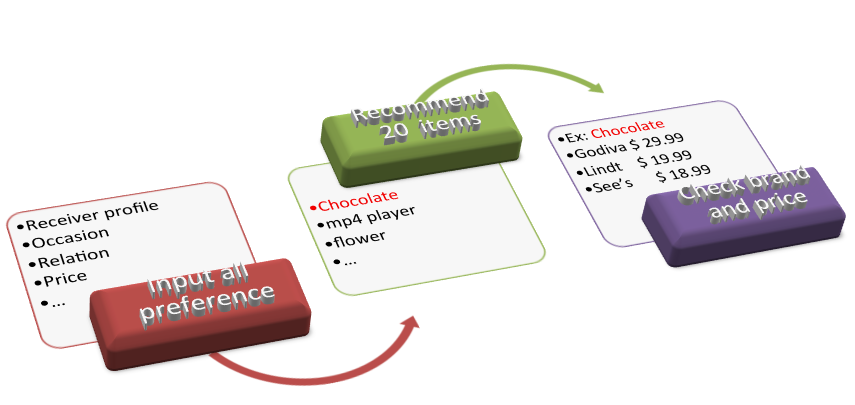
\includegraphics[width=\linewidth]{flow.png}
}
\caption{Flow Chart}
\end{figure}


\subsection{UI Design}
The UI of the GiftGiver is as below[picture2.1], it is a 1page website.   We separate the question in to 3 big part, the main consideration, the Receiver profile and the Result.   Sender can easily fill in their consideration step by step. 
After fill in the answer, system will comes out 20 recommended gifts.  If receiver are not satisfied, he/she can also change the answer and search again.

Compare to gifts website, our UI has a better flow but less option in some question.   For example, Gifts.com has 9 ages degree, such as 0~6, 7~12, 13~19, 20~30, 31~40 etc.   However, we prefer using fuzzy set to define our age instead of clear separation by years.   Because nouns like child, adult etc. will help the system in the commonsense part.  On the other hand, some people still looks like a child even that person has already more than 30s.  The fuzzy part will come out positive result.




\begin{figure}[h!t]
\centering{
    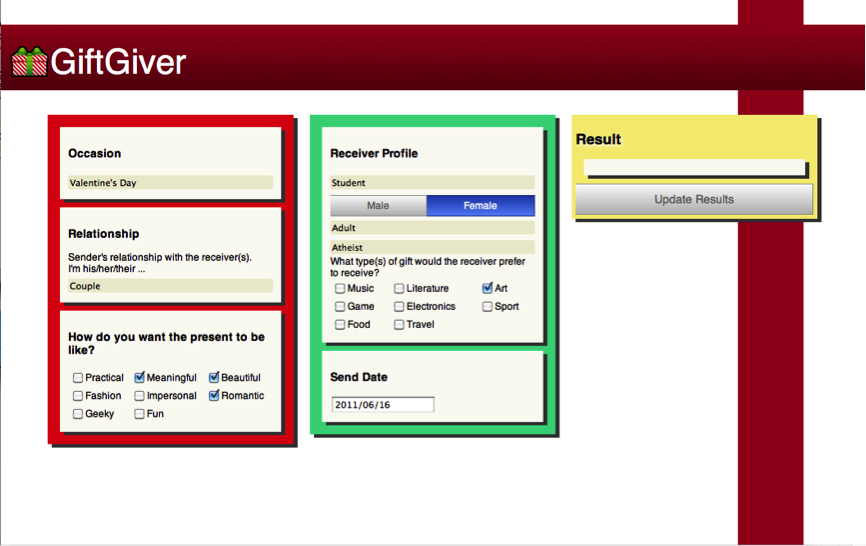
\includegraphics[width=\linewidth]{ui.png}
}
\caption{UI design}
\end{figure}

\subsection{Methodology}

Briefly explain our algorithms

\subsubsection{Feature Vectors}
As a recommendation system, we use a feature matching type of the recommendation system[韋狄再common sense報過的那邊survey paper].
We analyze 60 gifts items and 3 common occasions by 8 features.  
The features are:
1.[ Practical   ] – Is it functional or just for decoration?
2.[ Meaningful  ] – Is it has other meaning besides its function? 
3.[Beautiful    ] – Is it good looking?
4.[Trendy       ] – Is it fashion?
5.[Impersonal   ] – Is it just for him/her or other people can use it?
6.[Romantic ] – Is it present for love and sweet?
7.[Geeky        ] – Is it electrical?
8.[Fun      ] – Is it let you happy in a pure way?

Each gifts and occasion will have a vector of 8 features.  The value is normalized to[0,1].

Then the Vector will looks like below:
Gift     -> Book              [ 1.0, 0.6, 0.2, 0.4, 1.0, 0.0, 0.0, 0.6]
Occasion->Valentine’s day     [ 0.2, 1.0, 0.6, 0.2, 0.0, 1.0, 0.2, 0.2]




\subsubsection{Commonsense knowledge base}
In our system, we use Open Mind Common Sense, a knowledge corpus that contains 800,000 sentences about everyday life, gathered from Web volunteers. Using this resource, we successfully built a fashion recommendation system.

{\large ConceptNet}
ConceptNet aims to give computers access to common-sense knowledge, the kind of information that ordinary people know but usually leave unstated.
The data in ConceptNet is being collected from ordinary people who contributed it on sites likeOpen Mind Common Sense. ConceptNet represents this data in the form of a semantic network, and makes it available to be used in natural language processing and intelligent user interfaces.
ConceptNet is an open source project, with a Python implementation and a REST API that anyone can use to add computational common sense to their own project. A great tool to help you use ConceptNet in your software is Divisi.

\begin{figure}[h!t]
\centering{
    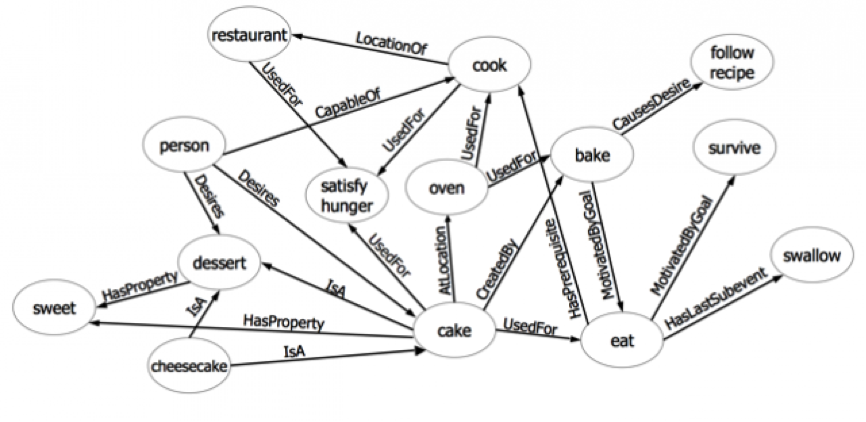
\includegraphics[width=\linewidth]{graph.png}
}
\caption{ConceptNet concept graph}
\end{figure}


{\large Divisi}
is a library for reasoning by analogy and association over semantic networks, including common sense knowledge.
Divisi uses a sparse higher-order SVD can help find related concepts, features, and relation types in any knowledge base that can be represented as a semantic network. By including common sense knowledge from ConceptNet, the results can include relationships not expressed in the original data but related by common sense.


\section{Evaluation}
It is rather hard to evaluate recommender system, and even so with common sense knowledge because there is no
common criterions to evaluate common sense. However, since we haven't found the state of the art recommender engine
using common sense for gift recommendation, we have conducted a couple surveys and user studies to evaluate the accuracy
of our recommender system.

Based on time constraints, we conducted a usability test and two surveys with five National Taiwan University graduate students and alumnae.
The results of the surveys and the usability test are listed below.

\begin{table*}[ht]
\caption{Usability test results}
\centering
\begin{tabular}{| p{5cm} | c | c | c | c | c |}
\hline
Question & Subject 1 & Subject 2 & Subject 3 & Subject 4 & Subject 5 \\
\hline
Was the UI easy to use? & 3 & 4 & 3 & 3 & 4 \\
\hline
Did the options cover all my considerations for gift recommendation? & 3 & 4 & 3 & 4 & 3 \\
\hline
Were the ideal gifts in the result list? & 4 & 4 & 3 & 4 & 4 \\
\hline
Were most of the recommendations realistic? & 5 & 3 & 3 & 5 & 4 \\
\hline
Was the price checking feature helpful? & 4 & 5 & 5 & 5 & 4 \\
\hline
Will you consider using our system for gift recommendation in the future? & 5 & 4 & 4 & 5 & 4 \\
\hline
\end{tabular}
\label{table:usetest}
\end{table*}

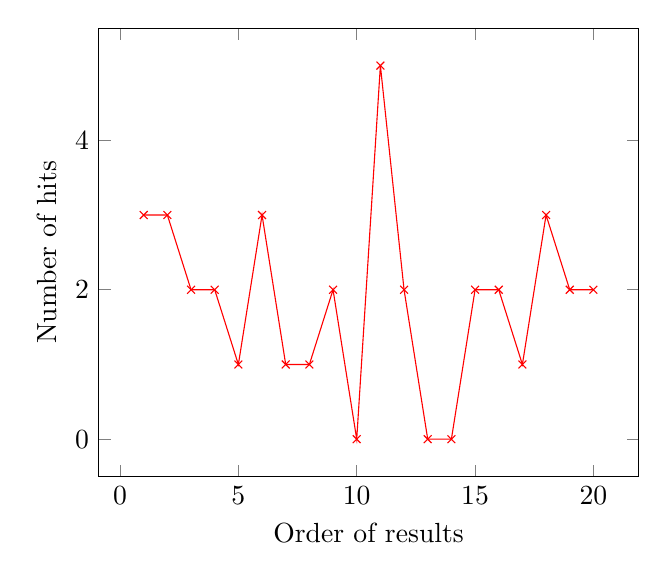
\begin{tikzpicture}
    \begin{axis}[xlabel=Order of results, ylabel=Number of hits]
    \addplot[color=red,mark=x] coordinates {(1,3) (2,3) (3,2) (4,2) (5,1) (6,3) (7,1) (8,1) (9,2) (10,0) (11,5) (12,2) (13,0) (14,0) (15,2) (16,2) (17,1) (18,3) (19,2) (20,2)};
    \end{axis}
\end{tikzpicture}

According to the plot above, the distribution is pretty even through out the search results but some bumpy hills along. We define hit rate as the number of times the tester's desired gift is ``hit'' on the result list. The higher the number the better our system performs. To illustrate the result of our survey in terms of hit rate, the scatter plot below provides the representation for that.

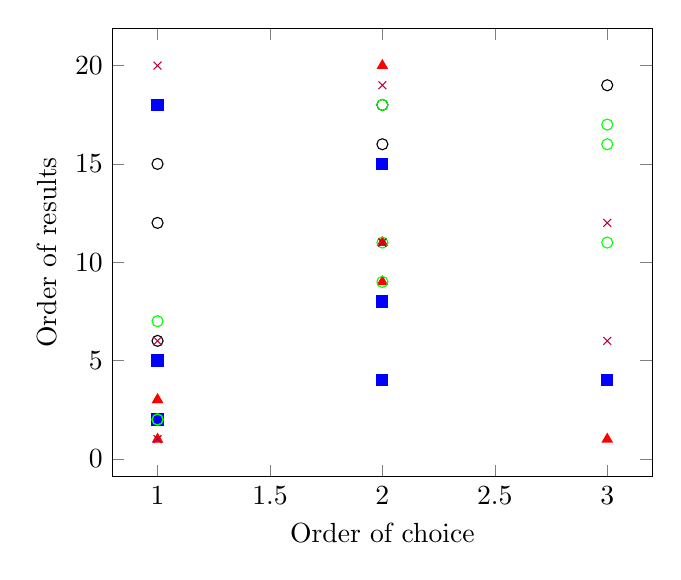
\begin{tikzpicture}
    \begin{axis}[
    xlabel=Order of choice,
    ylabel=Order of results,
    scatter/classes={
    a={mark=square*,blue},%
    b={mark=triangle*,red},%
    c={mark=o,draw=black},
    d={mark=o,draw=green},
    e={mark=x,draw=purple}
    }]
    \addplot[scatter,only marks,scatter src=explicit symbolic] 
    coordinates {
    (1, 5) [a]
    (2, 15) [a]
    (1, 18) [a]
    (2, 8) [a]
    (3, 4) [a]
    (1, 2) [a]
    (2, 4) [a]

    (1, 3) [b]
    (2, 20) [b]
    (1, 1) [b]
    (2, 9) [b]
    (1, 3) [b]
    (2, 11) [b]
    (3, 1) [b]

    (1, 15) [c]
    (1, 6) [c]
    (2, 18) [c]
    (3, 19) [c]
    (1, 12) [c]
    (2, 16) [c]

    (1, 7) [d]
    (2, 18) [d]
    (3, 16) [d]
    (1, 2) [d]
    (2, 11) [d]
    (3, 17) [d]
    (1, 2) [d]
    (2, 9) [d]
    (3, 11) [d]

    (1, 6) [e]
    (2, 11) [e]
    (3, 12) [e]
    (1, 1) [e]
    (2, 11) [e]
    (1, 20) [e]
    (2, 19) [e]
    (3, 6) [e]
    };
    \end{axis}
\end{tikzpicture}


\section{Conclusion}

A comparison of the approaches and contributions of the paper.
What is solved, what is left out.

\bibliography{aai2011}
\bibliographystyle{abbrv}



\end{document}
